 \documentclass[11pt, oneside]{article}   	% use "amsart" instead of "article" for AMSLaTeX format
\usepackage{geometry}                		% See geometry.pdf to learn the layout options. There are lots.
\geometry{letterpaper}                   		% ... or a4paper or a5paper or ... 
%\geometry{landscape}                		% Activate for for rotated page geometry
%\usepackage[parfill]{parskip}    		% Activate to begin paragraphs with an empty line rather than an indent
\usepackage{graphicx}				% Use pdf, png, jpg, or eps§ with pdflatex; use eps in DVI mode
								% TeX will automatically convert eps --> pdf in pdflatex		
\usepackage{amssymb}
\usepackage{amsmath}
\usepackage{parskip}
\usepackage{color}
\usepackage{hyperref}

\title{Quick Review}
%\author{The Author}
%\section{}
%\subsection*{}
\date{}							% Activate to display a given date or no date

\graphicspath{{/Users/telliott_admin/Dropbox/Tex/png/}}
% \begin{center} 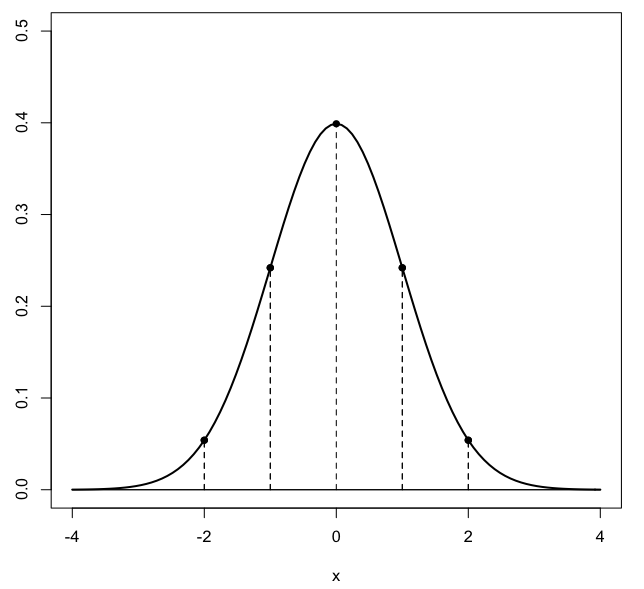
\includegraphics [scale=0.4] {gauss3.png} \end{center}
\begin{document}
\maketitle
\Large
\section*{Cauchy Integral theorem}
If we can write an integral in this form 
\[ I = \int_C \frac{f(z)}{z - z_0} \ dz \]
then the theorem says that
\[ I = 2 \pi i f(z_0) \]
\subsection*{examples}
\[ \int_C \frac{1}{z} \ dz = 2 \pi i \]
since the function is $f = 1$ (not $1/z$), and $f(0) = 1$.

\[ \int_C \frac{1}{z^2 + 1} \ dz \]
\[ = \int_C \frac{1}{(z - i)(z + i)} \ dz \]
\[ = \frac{1}{2i} \int_C \frac{1}{z - i} - \frac{1}{z + i} \ dz \]
If the contour includes either one of the points $i$ or $-i$, then there is a contribution of $2 \pi i$ toward the value of the integral from that point.  For example, the unit circle centered at $(0,i)$ gives $I = \pi$.

\subsection*{residues}
Another approach to the previous example is to say that the value of the integral is the $2 \pi i$ times the sum of the residues.  For a simple pole of order $1$, the residue is
\[ \text{Res} = \lim_{z \rightarrow z_0} (z - z_0) f(z) \]
So in the above example where only $z = i$ is included in the contour 
\[ \text{Res} = \lim_{z \rightarrow i} (z - i) \frac{1}{(z - i)(z + i)}  \]
\[ = \lim_{z \rightarrow i} \frac{1}{z + i} = \frac{1}{2i} \]
times $2 \pi i$ gives $I = \pi$.

\subsection*{derivatives}
Since
\[ 2 \pi i f(z_0) = \int_C \frac{f(z)}{z - z_0} \ dz \]
write
\[ 2 \pi i f'(z-z_0) = \int_C \frac{f(z)}{(z - z_0)^2} \ dz \]
\[ 2 \pi i f^n(z-z_0) = n! \ \int_C \frac{f(z)}{(z - z_0)^n} \ dz \]

\subsection*{examples}
\[ f(z) = \frac{1}{z(z-2)^2} \]
The first reside is just 
\[ \text{Res}(0) = \lim_{z \rightarrow 0} (z) \frac{1}{z(z-2)^2} \]
\[ = \lim_{z \rightarrow 0} (z) \frac{1}{(z-2)^2} = \frac{1}{4} \]
for the second pole, we need the derivative version.  First multiply by $(z-2)^2$
\[ (z-2)^2 f(z) = \frac{1}{z} \]
Compute the $N - 1$ derivative of what's left
\[ - \frac{1}{z^2} \]
Evaluate the limit as $z \rightarrow 2$
\[ - \frac{1}{4} \]
The residue is this result multiplied by $n! = 1$, and the value of the integral is $2 \pi i$ times the sum of the residues.  The result in this case is zero.

\section*{Laurent series}
Yet another way to work these problems is Laurent series.  That's our next stop.  But we can do a quick example.  If we have the series, we can just integrate the term with $(z-z_0)^{-1}$ because all the other terms are equal to zero.
\subsection*{examples}
Suppose
\[ f(z) = \frac{e^z}{z^2} \]
Since we know that 
\[ e^z = 1 + z + z^2 \dots \]
\[ f(z) = \frac{1}{z^2} + \frac{1}{z} + 1 + \dots \]
\[ \int_C f(z) \ dz = \int_C \frac{1}{z} \ dz = 2 \pi i \]
By the method of derivatives we would first multiply by $z^2$
\[ e^z \]
Compute the $N-1$ derivative of what's left 
\[ e^z \]
Evaluate the limit as $z \rightarrow 0 = 1$ and finally, multiply by $2 \pi i$.  The result is the same.  

Consider
\[ \exp \ (\frac{1}{z^2}) \]
We use the series for $e^z$ and substitute $z^2$
\[ = 1 + \frac{1}{z^2} + \frac{1}{2! z^4} + \dots \]
There is no term containing $z^{-1}$ and therefore the residue is zero, even though there is a pole (the function is undefined at $z = 0$).  Thus, even though the function is not analytic in a region containing the origin, the integral is zero.  This is an example of a "removable singularity."

\[ I = \int_C z^2 \sin (1/z) \ dz \]
The Maclaurin series for sine is
\[ \sin z = z - \frac{z^3}{3!} + \frac{z^5}{5!} - \dots \]
\[ \sin1/ z = 1/z - \frac{1}{3! \ z^3} + \frac{1}{5! \ z^5} - \dots \]
Multiplying by $z^2$:
\[ I = \int_C z - \frac{1}{3! \ z} +  \frac{1}{5! \ z^3} - \dots \]
Here we do have a term with $1/z$ and its coefficient is $1$.  So the residue is $-1/3!$ and the value of the integral is $- \pi i/3$.

An example from Brown is 
\[ \frac{1}{z(z-2)^4} \]
Since their example is about Laurent series, they do the following.  Rewrite
\[ \frac{1}{z} = \frac{1}{2 + (z - 2)} \]
to go with the other factor.  Then
\[ = \frac{1}{2} \cdot \frac{1}{1 - (- \frac{z - 2}{2})} \]
So we have a factor of $1/2(z-2)^4$ multiplying something that can be expanded using the geometric series to give
\[ 1 + (-\frac{z - 2}{2}) + (-\frac{z - 2}{2})^2 + (-\frac{z - 2}{2})^3 \dots \]
The only term that gives us anything like $z^{-1}$ after multiplying by $1/2(z-2)^4$ is the last one:
\[ \frac{1}{2} \cdot \frac{1}{(z-2)^4} \cdot (-\frac{z - 2}{2})^3 = - \frac{1}{16} \frac{1}{(z-2)}   \]
The coefficient is $-1/16$ which multiplies $2 \pi i$ to give $-\pi i/8$.

We did this problem by the method of residues at the end of Chapter 19 in the main write-up.

\section*{Quotients}
Brown and Churchill put it this way.  Suppose we have the function $p/q$ where both $p$ and $q$ are both analytic at a point $z_0$. Suppose also
\[ q(z_0) = 0 \]
\[ p(z_0) \ne 0 \]
and
\[ q'(z_0) \ne 0 \]
Then $z_0$ is a simple pose of the compound function and
\[ \text{Res} (z_0) = \frac{p(z_0)}{q(z_0)} \]

\subsection*{example}
\[ \cot z = \frac{\cos z}{\sin z} \]
The zeroes of $\sin z$ occur at $n \pi$ so each point $z = n \pi$ of $f$ is a simple pole.  But $q'(z) = p(z)$ so the residue at these poles is just $1$.

\end{document}  
